\documentclass[a4paper, 11pt]{article}
% ----- Loading the Package MCMthesis -----
% -----           v 5.01-L            -----
% `tcn' is short for `Team Control Number'.
% You should fill your tcn after the equal sign following tcn.
% The option `sheet' contorls weather the summary sheet
% will appear.
% The option `abstract' controls weather the abstract 
% will appear in the title-page.
\usepackage[tcn = 28218, sheet = true, abstract = false]{MCMthesis}
% ----- Question Mark -----
\problem{A}
% ----- Fonts settings -----
% You may need to install the font files, if it's needed.
% Disable it, if you don't want this font.
\usepackage{palatino}
% ----- Set the skip betweent the paragraphics -----
\setlength\parskip{.5\baselineskip}
% ----- The name of Abstract ------
\providecommand{\abstractname}{\relax} % <-- Do not modify here.
\renewcommand{\abstractname}{Abstract} % <-- Modify here, if needed.


% -----------------------------------
% ===== The Title of Your Paper =====
% -----------------------------------
\title{title}
% ---------------------------------------
% ===== The Author(s) of Your Paper =====
% ---------------------------------------
% ----------------
% ===== Time =====
% ----------------
\begin{document}
% Abstract should be put before 
\begin{abstract}
Traffic rule has a great impact on the efficiency and safety of a traffic system. Thus to build a model to evaluate the rule is of great importance. In most countries, there exists such a rule: unless overtaking another car, drivers are supposed to drive on the right-most lane. In our passage, we are trying to develop a model to evaluate this rule from two aspects: the traffic flow and the safety.
We construct a blank situation that is without the right-most rule. Using our model, we compare the safety and the traffic flow under the two situation, with the right-most rule and without the right-most rule.

To evaluate the safety, we build a model to calculate the safety distance. If the distance between two car is less than the safety distance. The collision will happen. The less the probability of the collision is, the safer. So we use the probablity of the collision to evaluate the

\begin{keywords}
keyword1; keyword2
\end{keywords}
\end{abstract}
\maketitle
\pagestyle{empty}
\newpage
% Generate the Table of Contents, if it's needed.
\tableofcontents
\newpage
\pagestyle{fancy}
% The body of your paper

% ==============================================================
% Introduction
% ==============================================================

\section{Introduction}

In bidirectional traffic, right- and left-hand traffic requires 
vehicles keep either to the right or the left side of the road, 
respectively.\cite{Draper_Geoff_1993} The first right-hand 
traffic law in United State dates back to 1792, applied to the 
Philadelphia and Lancaster Turnpike.
\cite{Weingroff_Richard_2014}\\

The right-hand traffic rule derives regulations on multi-lane 
freeways, which often requires drivers to drive in the 
right-most lane unless they are passing another vehicle, in 
which case they move one lane to the left, pass, and return 
to their former travel lane. The overtaking lane provides 
redundant convenience and safety for vehicles to pass others, 
but lowers freeway's traffic flow capability.\\

Different models may exist that provide a better trade-off 
among traffic flow, safety and convenience. This paper 
considers these three criteria, introduces a different 
freeway traffic model and analyses performances of the two 
models.



% ==============================================================
% Modeling
% ==============================================================

\section{Performance Evaluation}

Performance of a traffic rule is determined by the three 
criteria below: 

\paragraph{Safety} Distance and braking capability of adjacent 
vehicles, and speed limits of the road, together affects the 
safety. \textbf{Safety factor $\alpha$} is a value to measure 
how safe a vehicle is, and its value can be calculated from 
a safety evaluation function discussed at the next section.

\paragraph{Traffic Flow} xxxxxxxxx

\paragraph{Convenience} xxxxxxx


\section{Safety Factor}

\emph{Assumptions}

The value of acceleration subjects to normal distribution, 
$\mu = \frac{max(a)}{2}$, $\sigma = \frac{1}{4}\mu$, for 
$p(0 < a_2 < \frac{1}{4} \mu)$ and 
$p(\frac{7}{4} \mu < a_2 < 2\mu)$ is very small.

\subsection{Safe Distance Model}

On the highway, if the car in front suddenly slows down, 
it is likely that a car crash happens. We build this model 
to calculate the safe distance between two adjacent cars. 
That is, if the adjacent $d \leq l$ and the car in front 
suddenly slows down,the accident will not happen.\\ \\

\begin{table}
\centering
\begin{tabular}{ll}
\hline
Parameter & Description\\
\hline
$a_1$ & the acceleration of the  car in behind \\
$v_1$ & the velocity of the  car in front \\
$a_2$ & the acceleration of the car in front \\
$v_1$ & the velocity of the  car in front \\
$t_r$ & the driver's reaction time \\
$t$ & the total time whole process \\
$l$ & the safe distance \\
$d$ & a constant which is the real distance between the 
car in front and the car in behind.\\
\hline
\end{tabular}
\caption{Model parameter}
\end{table}

\begin{figure}[h]
\small
\centering
\includegraphics{situation.png}
\caption{}
\end{figure}

There are two possible situations that the accident will 
happen:
\begin{itemize}
\item The accident happens after the car in front stopped.
That is, when
\begin{displaymath}
\frac{v_2}{a_2}  \geq  \frac{v_1}{a_1} + t_r
\end{displaymath}
We have:
\begin{eqnarray}
\frac{v_1^2 - v_0 ^ 2}{2a_1} + v_1 t_r - l & = & \frac{v_2 ^ 2 - v_0 ^ 2}{2a_2}\\
\frac{v_2 - v_0}{a_2} & = & t\\
\frac{v_1 - v_0}{a_1} & = & t - t_r
\end{eqnarray}
\item The collision happens before the car in front stopped. 
That is, when
\begin{displaymath}
\frac{v_2}{a_2}  >  \frac{v_1}{a_1} + t_r
\end{displaymath}
We have:
\begin{eqnarray}
v_1 t_r + \frac{v_1 ^ 2}{2a_1} - l& = &\frac{v_2^2}{2a_2}
\end{eqnarray}
\end{itemize}

Solve this equation array, we have
\begin{displaymath}
l(a_1, a_2, v_1, v_2) = 
\left \{
\begin{array}{cl}
\dfrac{(a_1a_2t_r^2 + 2a_1t_rv_2 + v_1^2 - 2v_1v_2 + v_2^2)}{2(a_1-a_2)} & \dfrac{v_2}{a_2}  \geq \dfrac{v_1}{a_1} + t_r \\
v_2 t_r + \dfrac{v_1 ^ 2}{2a_1} -\dfrac{v_2^2}{2a_2} & \dfrac{v_2}{a_2}  < \dfrac{v_1}{a_1} + t_r
\end{array}
\right .
\end{displaymath}
\\

To calculate $l_{max}$, firstly, we are going to find the extrema,

\begin{displaymath}
\left \{
\begin{array}{cl}
\dfrac{\partial l}{\partial{a_1}} = 0 \\
\dfrac{\partial l}{\partial{a_2}} = 0 \\
\dfrac{\partial l}{\partial{v_1}} = 0 \\
\dfrac{\partial l}{\partial{v_2}} = 0 \\
\end{array}
\right .
\end{displaymath}

This equation array has no solution, which indicates that we can 
get the $l_{max}$ at the boundary of domain.

$l$ reaches the maximum when $a_1$ equals to $a_{min}$, { }$v_1$ 
equals to $v_{1max}$, $v_2$ equals to $v_{2min}$. (If the front 
car drives with the lowest speed, the rear car drives with the 
highest speed, and at the same time, rear car's acceleration is 
the minimum, when emergency happens, the braking distance is 
the longest.)

Thus,
\begin{displaymath}
l_{max}(a_2) = 
\left \{
\begin{array}{cl}
\dfrac{(a_{min}a_2t_r^2 + 2a_{min}t_rv_{min} + v_{max}^2 - 2v_{max}v_{min} + v_{min}^2)}{2(a_{min}-a_2)} & \dfrac{v_{min}}{a_2}  \geq \dfrac{v_1}{a_1} + t_r \\
v_{min} t_r + \dfrac{v_{max} ^ 2}{2a_{min}} -\dfrac{v_{min}^2}{2a_2} & \dfrac{v_2}{a_2}  < \dfrac{v_1}{a_1} + t_r
\end{array}
\right .
\end{displaymath}\\

\paragraph{$l${ } Distribution}
From the result above, we can get $a_2(l)$

%\usepackage{amsmath}
\[ a_2(l) = \begin{cases}
-\dfrac{v_{max}^2 - 2v_{max}v_{min} + 2a_{min}t_rv_{max} + v_{min}^2 - 2a_{min}t_rv_{min} - 2la_{min}}{a_{min}t_r^2 + 2l}, 
\\

\quad l \leq \dfrac{v_{max}^2 - v_{max}v_{min} + 2v_{max}a_{min}t_r - a_{min} v_{min}t_r}{2a_{min}}\\
\dfrac{a_{min}v_{min}^2}{v_{max}^2 + 2a_{min}t_rv_{max} - 2la_{min}}, \quad  l > \dfrac{v_{max}^2 - v_{max}v_{min} + 2v_{max}a_{min}t_r - a_{min} v_{min}t_r}{2a_{min}}
\end{cases}\]
\\

\paragraph{Safety Factor $\alpha$}
For every car, it has a unique safety factor $\alpha$, the 
closer the distance between two adjacent cars is, the smaller 
the $\alpha$ is, vice versa.\\

\begin{figure}[h]
\small
\centering
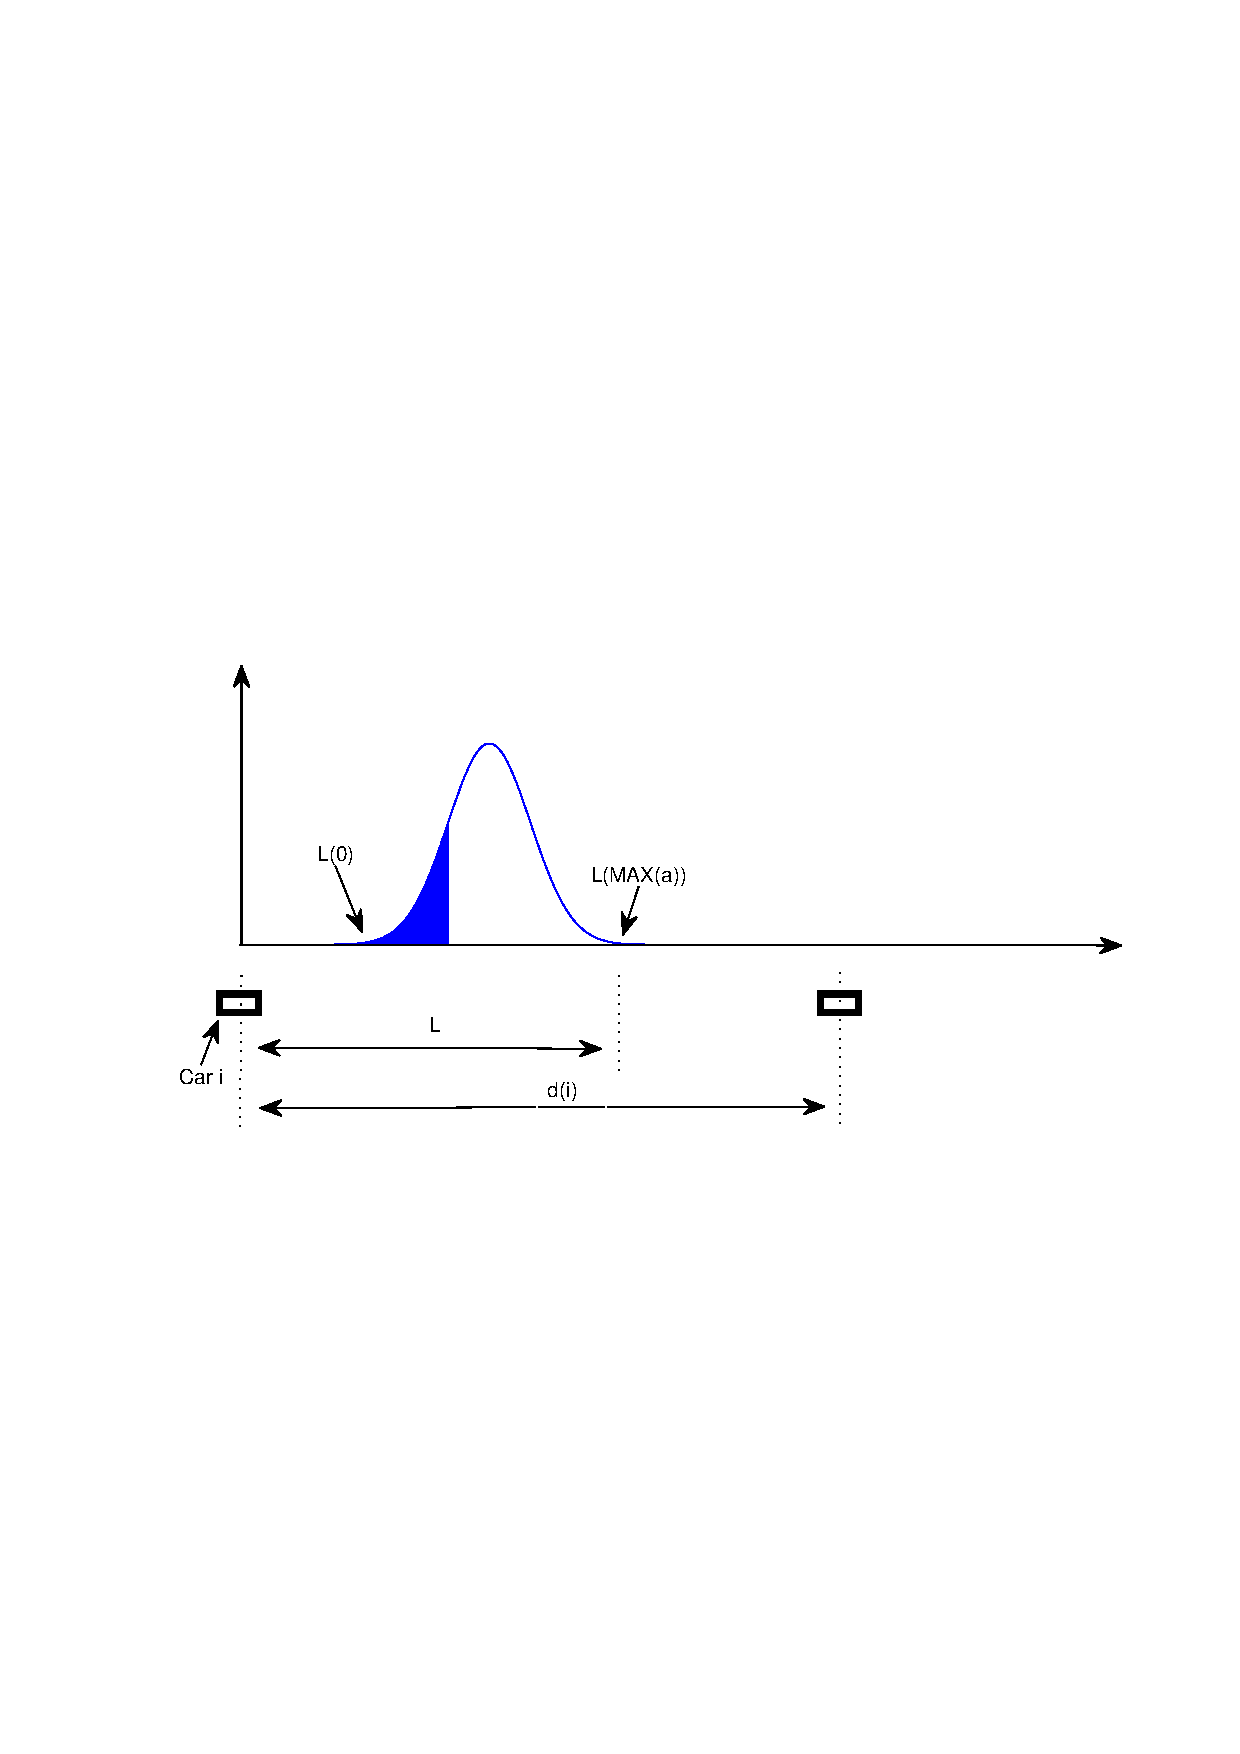
\includegraphics{draw_SafetyNormalDistribution_graph.png}
\caption{safety factor distribution} \label{fig::safety factor distribution}
\end{figure}
\begin{displaymath}
\alpha(l) = \int_{0}^{l} f(x) dx.
\end{displaymath}
%\textbf{Assumptions}\\
%\begin{itemize}
%\item d is the distance between two adjacent cars.
%\end{itemize}
We can see that , when $a_2$ = 0, that is, the front car 
has the lowest deceleration. Since $l(a)$ is a monotone 
increasing function, at this time,$l$ is minimal. In other 
word, it is of little possibility that the distance is less 
than the l, that is, $\alpha(l) \rightarrow 0$                     


\section{Traffic Flow Factor $\beta $}
\emph{Assumption}

\begin{itemize}
\item $v$ and $\rho$ suits the Greenshield Model
%\item 车道上车的密度较小的时候,车的行驶
\end{itemize}

\begin{table}
\centering
\begin{tabular}{ll}
\hline
Parameter & Discription\\
\hline
$\rho $ & The traffic density\\
$\rho_j$ & The traffic density under the traffic jam condition\\
$\rho_m$ & The traffic density when the the traffic flow is the highest.\\
$v_f$ & The velocity of the vehicle when the traffic density is small \\
$Q$ & Traffic flow \\
%$N$ & The total number of the car on the freeway
\hline
\end{tabular}
\caption{Model parameter}
\end{table}

\paragraph{The relationship between $v$ and $\rho$ }
According to the Greenshield Model, the $v $and $\rho$ has such a 
relationship:

\begin{equation}
v = a - b\rho
\end{equation}
$a$ and $b$ are coefficients

\begin{itemize}
\item let $\rho = 0$,$v = v_f$,
we have $a = v_f$
\\
\item when the traffic density is highest, that is,
$\rho = \rho j$, $v = 0$,
we have $b = \frac{v_f}{k_j}$
\end{itemize}

Therefore, we have 
\begin{equation}
v = v_f(1 - \frac{\rho}{\rho_j})
\end{equation}

\begin{equation}
\rho = \rho_j(1 - \frac{v}{v_f})
\end {equation}

\paragraph{The relationship between $Q$ and $\rho$ }
\begin{equation}
Q = \rho v = v_f(\rho - \frac{\rho^2}{\rho_j})
\end{equation}
This function has such properties:

\begin{itemize}
\item $Q$ is a quadratic function. 
\item when $\frac{dQ}{d \rho} = 0$, 
$\rho = \frac{1}{2}\rho_j = \rho_m $
What's more, it passes through the origin.
\end{itemize}
%Since the layout of the cars on the freeway is complicated, 
%to simplify, we use a special model to discuss the 
%relationship between the safety and traffic flow under the 
%situation with and without the right-most rule.
%\paragraph{Assumption}

%\begin{itemize}
%\item the rest flow on a single lane drive with a constant speed.

%\subsection{Con Model}
%\paragraph{Assumption}
%\begin{itemize}
%\item Only one car are overtaking, the others are driving with a constant speed
%\item Every overtaking, pass only one car
%\end{itemize}

\begin{equation}
J^* = J_{supply} - J_{need}
\end{equation}

\[ J^* = \begin{cases}
0,\\
\bar{l} - \bar{l}_{max}
\end{cases}\]

%\item Without the right-most rule, there is no overtaking lane, vehicle can stay on either lane at any time.
%\item On the freeway, except the overtaking car, others are subject to the uniform distribution.
%\end{itemize}


\begin{displaymath}
\beta = A\beta_1 + B\beta_2
\end{displaymath}

%\begin{itemize}
%\item 
%\begin{displaymath}
%\beta_1 = \frac{J_1 - J_2}{J_2}
%\end{displaymath}
%\end{itemize}



\section{Convenience Factor}
\emph{Assumption}
\begin{itemize}
\item We only consider the two-lane freeway's overtaking situation.
\end{itemize}
Without the right-most rule, a vehicle can drive on both lane for a long time, which indicates that the possibilities that one car block another car will increase.
在没有了向右行驶的规则之后,一辆车可以长时间停在左边车道或是右边车道。遮挡的情况变得普遍出现于没有该规则的道路上。遮挡的时间越多,
超车越困难,也就是说越不方便。XXXXX
所以,遮挡可以作为衡量道路情况的一个指标
\emph{Assumption}
\begin{itemize}
\item The traffic density is uniform distribution
\end{itemize}

% ==============================================================
% Analysis
% ==============================================================

\section{Model Analysis}


% ==============================================================
% Conclusions
% ==============================================================

\section{Conclusions}



% ==============================================================
% Discussion
% ==============================================================

\section{Discussion}

\subsection{Strengths}
	
\subsection{Weaknesses}



% ==============================================================
% References
% ==============================================================

\begin{thebibliography}{99}

\bibitem{Draper_Geoff_1993} Draper, Geoff (1993). "Harmonised 
Headlamp Design for Worldwide Application". Motor Vehicle 
Lighting. Society of Automotive Engineers. pp. 23-36.

\bibitem{Weingroff_Richard_2014} Weingroff, Richard. "On The 
Right Side of the Road". United States Department of 
Transportation. Retrieved 10 January 2014.

\bibitem{Mick_Hamer_1986} Left is right on the road', Mick Hamer 
New Scientist, 25 December 1986 - 1 January 1987 No 1540/1541, 
p.16.

\end{thebibliography}

\end{document}
% ----- End of Document Body -----